Die Geometrie und einige Stoffeigenschaften sind durch die in \ref{chap: wettingTheory} definierten vereinfachungen und Annahmen bereits vorgegeben. Im folgen wird zu beginn die Geometrie der Kapillare vorgestellt, gefolgt von den Materialeigenschaften und verwendeter Randbedingunen. Da mehrere Untersuchungen unternommen wurden, erfolgt in Kapitel eine Übersicht über die durchgeführten Simulationen und dessen Initialiserung. 


Wie bereits in Kapitel \ref{chap: Introduction} geschrieben, erfolgen die Simulationen mit dem solver \texttt{phaseFieldFoam}. Dieser wurde bereits mehrfach Validiert, worauf in Kapitel \ref{chap: Validation} genauer eingegangen wird.
\section{Geometry}
Die Geometrie der Kapillare wird so angenommen, dass sie wie in Abbildung \ref{fig: Capillary Geometry} zu sehen ein Reservoir mit Wasser hat, welches durch Oberflächeneffekte in die Kapillare strömt. Durch die Annahme, dass sich ein Teil des Wassers bereits in der Kapillare befindet, wird in der Simulieren Geometrie lediglich die Randbedingung so gesetzt, dass das Wasser in diesem Reservoir nachströmen kann. Die Dimensionen der Kapillare ergeben sich daraus, dass die Simulation der Kapillare perspektivisch auch mit experimenten verglichen werden soll. Daher wurden auch weitere, komplexere Geometrien simuliert, die jedoch nciht Teil dieser Arbeit sind. 
Wie zu erkennen, handelt es sich um eine Kapillare mit lediglich $6nm$ Durchmesser. Eine Simulation so kleiner Kapillare wurde soweit bekannt bisher nicht mit der Phasenfeld methode Simuliert.

\begin{figure}[h]
    \centering
    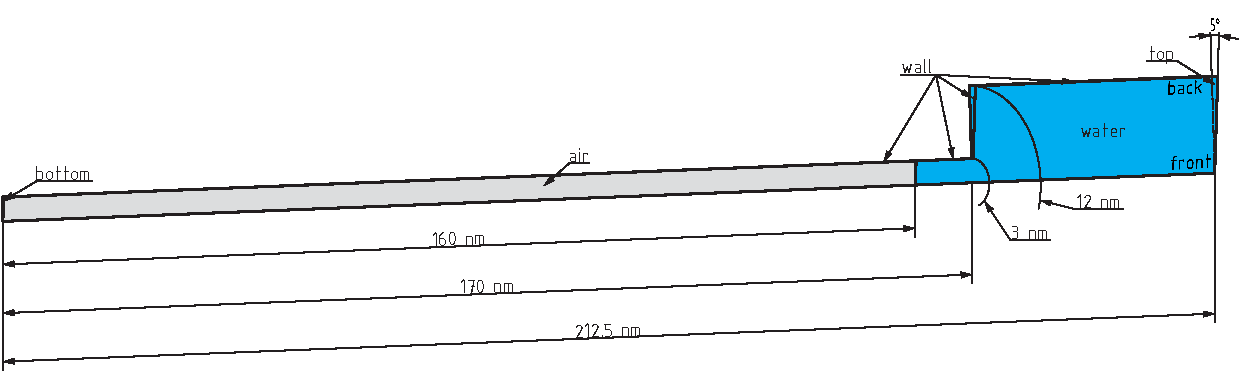
\includegraphics[width=.95\textwidth]{Pictures/Cap_5DEG.pdf}
    \caption{Schematic of used Capillary}
    \label{fig: Capillary Geometry}
\end{figure}

Die Diskretisierung der Geometrie wurde so gewählt, dass die Elemente eine Kantenlänge von $0.2nm$ haben. In Radialer Richtung hat eine Wedge nur ein Element. Zur erstellung der \texttt{blockMeshDict}-datei, wurde ein python skript erstellt, welches anhand des Kapillardurchmessers und länge eine Datei mit den in Abbildung \ref{fig: Capillary Geometry} dargestellten Benennungen der Oberflächen erstellt. 

\section{Randbedingunen}
In Abbildung \ref{fig: Capillary Geometry} sind neben der Geometrie auch die Flächen, die mit Randbedingungen versehen wurden benannt. Die Flächen \texttt{front} und \texttt{back} sind sich gegenüberliegende Flächen der Wedge und müssen dementsprechende Ranbedinungen erhalten. Die \texttt{wall} Flächen sind nicht durchdringbare Oberflächen und \texttt{top}, bzw. \texttt{bottom} Oberflächen durch die ein Fluss zugelassen wird.
Die wesentlichen Randbedingunen an der Wand sind in Tabelle \ref{tab: BoundaryConditions_wall} aufgelistet. 

\begin{table}[h]
    \centering
        \caption{relevant boundary conditions wall}
        \label{tab: BoundaryConditions_wall}
        \begin{tabular}{lll}
            Parameter & Value \\ \hline
            orderparameter $C$ & \texttt{equilibriumPhaseContactAngle}     \\
            equilibrium contact angle $\theta_{\mathrm{e}}$ & $15^{\circ}$, $45^{\circ}$, $75^{\circ}$\\
            chemisches Potential $\phi$   & \texttt{zeroGradient}        \\ 
            velocity $\mathbf{u}$ &   $\mathbf{u_{\mathrm{w}}} = 0$\\
            pressure $p$&  \texttt{fixedFluxPressure} \\
        \end{tabular}
\end{table}
Für den Ordnungsparameter $C$ wird die Gleichgewichtsrandbedingung angenommen und der Gleichgewichtskontaktwinkel für jede der drei Simulationen mit dieser Geometrie mit $15^{\circ}$, $45^{\circ}$ bzw. $75^{\circ}$ angegeben. Der Gradient des chemischen potentials an der Wand wird als null gesetzt, genauso wie die Geschwindigkeit der Wand. Die Ranbedingung für den Druck wird mit \texttt{fixedFluxPressure} so gewählt, dass der Druckgradient so angepasst wird, das der Massenfluss am Rand mit der vorgegebenen Geschwindigkeit an der Wand übereinstimmt. 

\section{Materialeigenschaften}
Für die Simulation werden unter anderem Wasser und Luft bei $25^{\circ}$ Celsius als Medium angenommen. Damit folgen die in Tabelle \ref{tab:physicalProperties_CaseSetup} dargestellten Materialeigenschaften. 
\begin{table}[h]
    \centering
    \caption{Physical properties}
    \label{tab:physicalProperties_CaseSetup}
    \begin{tabular}{lll}
    fluid & density ($\frac{kg}{m^3}$) & kinematic viscosity $\frac{m^2}{s}$ \\ \hline
    water & $1000$                     & $1.00E-06$                          \\
    air   & $1$                        & $1.00E-05$                          \\ 
    \end{tabular}
    \end{table}


\section{Simulationsparameter}

\subsection{function objects}


\section{Auswertungsmethoden}
Zur Auswertung der Simulation wurde unter anderem die Anwendung \texttt{paraview} verwendet. Alle bilder der Simulation wurden damit erzeugt. Die Auswertung und darstellung abgeleiteter oder berechneter Größen in Diagrammen wurden hingegen mit der python bibliothek \texttt{Matplotlib} erzeugt. Dazu wurde ein skript erstellt, das die Ergebnisse der function obsjects sammelt und gegebenenfalls Berechnungen damit vornimmt. 
